\chapter{ State of the art }
\setcounter{secnumdepth}{3}
\newpage

\section*{Introduction}
\addcontentsline{toc}{section}{Introduction}
This chapter will present and study various concepts such as Automation, Web Scraping, Version Control, DevOps, State Machine with an emphasis on the DevOps terminology such as the CI/CD pipelines. We will talk about the most used tools in the market as well as which ones we settled on after making a comparison.

\section{Automation \& Web Scraping concepts}
\addcontentsline{toc}{section}{Automation & Web Scraping concepts}
\subsection{Automation}
At its core, automation is leaving menial and recurring tasks to the automaton (or machine) in order to do more meaningful work as a human in the meantime. Implementing automation improves the efficiency, reliability and the speed of tasks that previously took humans a lot of time.
\subsection{Web Scraping}
Web scraping is the process of automatically extracting content and data from a website. Although data extraction is done in a brute way by reading texts from HTML elements, it is used in a variety of legitimate digital businesses like search engines, price comparison sites and market research companies. So contrary to what some might think, web scraping is completely legal.
\subsection{Relationship between the two}
Web scraping simplifies the process of extracting data and the automation process helps repeating the recurring task of extraction. As a result, the combination of scraping data, storing it and automating the whole process is getting very popular, especially with new technologies and tools arising in order to do just that.

\newpage
\section{DevOps}
\addcontentsline{toc}{section}{DevOps}
\subsection{Definition}
DevOps is the set of practices, techniques and tools used to speed up the Software Development Lifecycle (SDL) by bringing together two historically separate functions of development and operations. 

\medskip
Development refers to writing code and software, whereas operations refer to provisioning servers, configuring them as well as deploying the apps to them, amongst other things.

\medskip
DevOps teams focus on automating all of the above. The key terminologies around DevOps are Continuous Integration, Continuous Delivery and Infrastructure As Code (IAC).
\subsection{Lifecycle}
\begin{center}
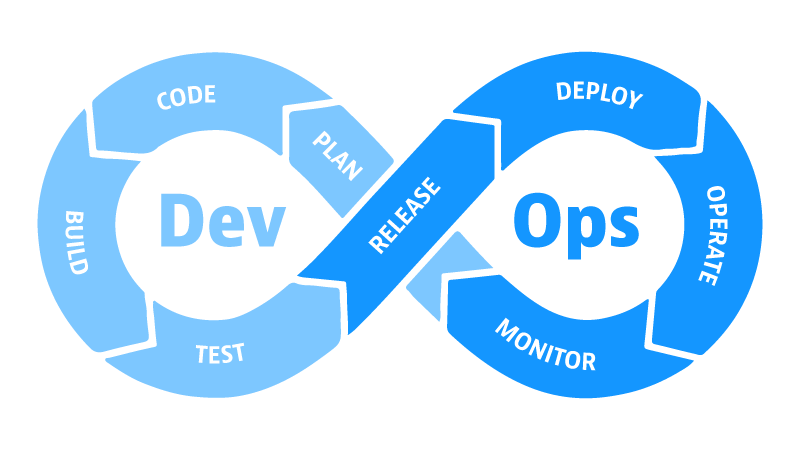
\includegraphics[width=9cm, height=5cm]{src/assets/images/devops.png}
\end{center}
\subsection{Container management}
Containers have become an integral part of DevOps over the past couple of years but what is a container exactly and how do we manage them? 
\subsubsection*{What is a container ?}
Simply said; container is a packaging format for software applications that are akin to a very lightweight virtual machine which always executes in an isolated environment. What this implies is that said containers can be easily copied to and run on different machines with high reliability, lower costs and high efficiency.
\subsubsection*{What is container management ?}
Container management is the process for automating the creation, deployment and scaling of containers. Container management tools such as Docker and Podman facilitate the addition, replacement and organization of containers.

\section{Microservices}
\addcontentsline{toc}{section}{Microservices}
\subsection{Definition}
Microservices are an architectural and organizational approach to software development where software is composed of small independent services that communicate over well-defined APIs. These services are owned by small, self-contained teams.

\medskip
Microservices architectures make applications easier to scale and faster to develop, enabling innovation and accelerating time-to-market for new features.
\begin{center}
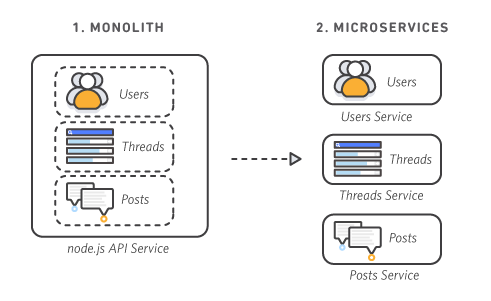
\includegraphics[width=10cm, height=7cm]{src/assets/images/microservices.png}
\end{center}
\subsection{Characteristics of Microservices}
\begin{itemize}
	\item \textbf{Autonomous :} Each component service in a microservices architecture can be developed, deployed, operated, and scaled without affecting the functioning of other services. Services do not need to share any of their code or implementation with other services. Any communication between individual components happens via well-defined APIs.
	\item \textbf{Specialized :} Each service is designed for a set of capabilities and focuses on solving a specific problem. If developers contribute more code to a service over time and the service becomes complex, it can be broken into smaller services.
\end{itemize}

\subsection{Benefits of Microservices}
\begin{itemize}
	\item \textbf{Agility :} Microservices foster an organization of small, independent teams that take ownership of their services. Teams act within a small and well understood context, and are empowered to work more independently and more quickly.
	\item \textbf{Flexible Scaling :} Microservices allow each service to be independently scaled to meet demand for the application feature it supports. This enables teams to right-size infrastructure needs, accurately measure the cost of a feature, and maintain availability if a service experiences a spike in demand.
	\item \textbf{Easy Deployment :} Microservices enable continuous integration and continuous delivery, making it easy to try out new ideas and to roll back if something doesn’t work. The low cost of failure enables experimentation, makes it easier to update code, and accelerates time-to-market for new features.
	\item \textbf{Technical Freedom :} Microservices architectures don’t follow a “one size fits all” approach. Teams have the freedom to choose the best tool to solve their specific problems. As a consequence, teams building microservices can choose the best tool for each job.
	\item \textbf{Reusable Code :} Dividing software into small, well-defined modules enables teams to use functions for multiple purposes. A service written for a certain function can be used as a building block for another feature. This allows an application to bootstrap off itself, as developers can create new capabilities without writing code from scratch.
	\item \textbf{Resilience :} Service independence increases an application’s resistance to failure. In a monolithic architecture, if a single component fails, it can cause the entire application to fail. With microservices, applications handle total service failure by degrading functionality and not crashing the entire application.
\end{itemize}

